\section{Situazioni Problematiche}

\begin{frame}{Punti Critici}
  Sono state incontrate diverse criticità, ad esempio:
  \begin{itemize}[<+- | alert@+>]
    \item{Gestione del ciclo delle fasi}
          \begin{itemize}
            \item Non è possibile "resettare" i processi
          \end{itemize}
    \item Organizzazione e aggiornamento sullo stato dei lavori di proposte autogestite
          \begin{itemize}
            \item Risolvibile con l'elezione di un responsabile
          \end{itemize}
    \item Gestione dell'autenticazione
  \end{itemize}

\end{frame}
\begin{frame}{Autenticazione}
  Decidim supporta la gestione dei permessi per i singoli componenti/fasi

  Una di queste prende il nome di \emph{Verifica delle autorizzazioni}

  \begin{wrapfigure}{r}{0.50\textwidth}
    \centering
    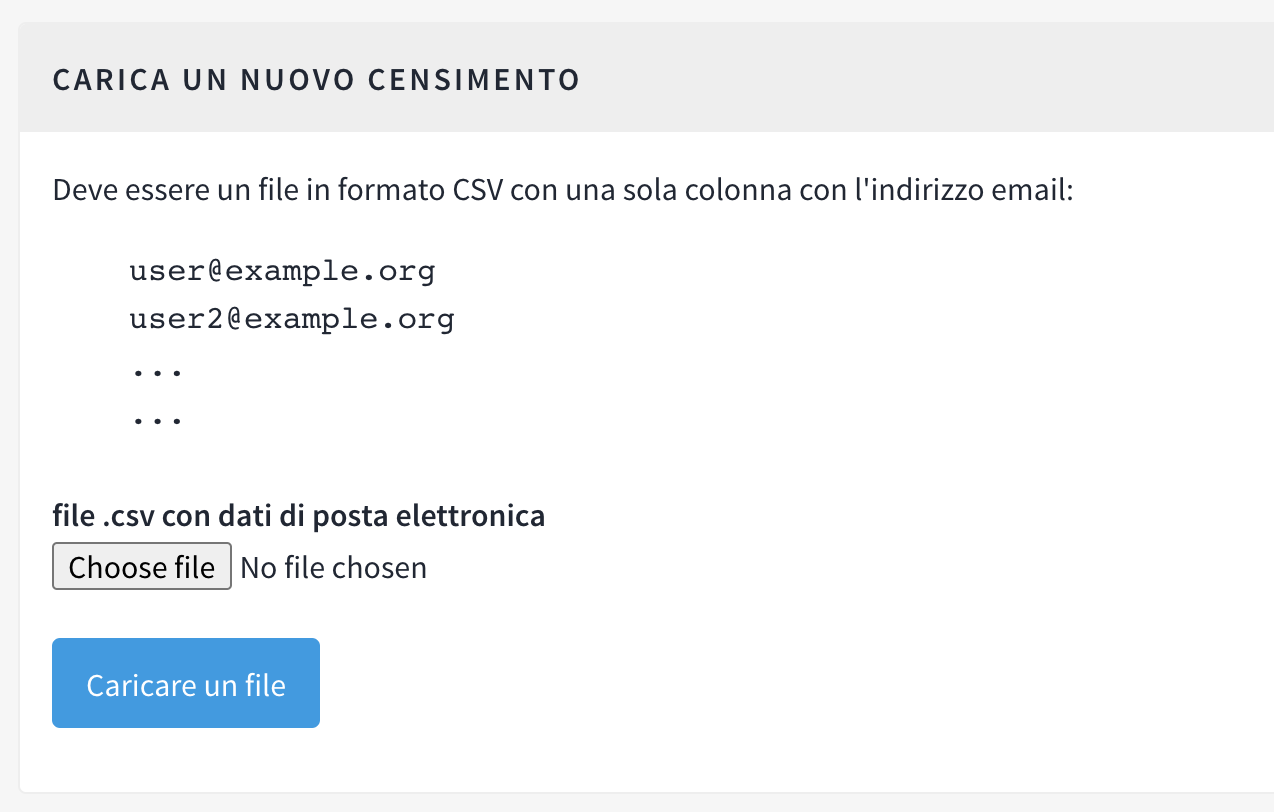
\includegraphics[width=0.50\textwidth]{images/auth}
  \end{wrapfigure}

  Per gestire l'autenticazione si potrebbe importare all'interno di Decidim una lista di mail possedute dall'azienda.

  (ad esempio quelle registrate all'interno degli "sportelli" online dell'azienda e quindi validate)

\end{frame}